\section{Categories of Urban Heat Island}
	
	There are two types of urban heat island based on how they are formed and how high they reach:
	surface urban heat islands and atmospheric urban heat islands (Figure \ref{fig:urban-heat-types}).
	
	\begin{figure}
		\centering
		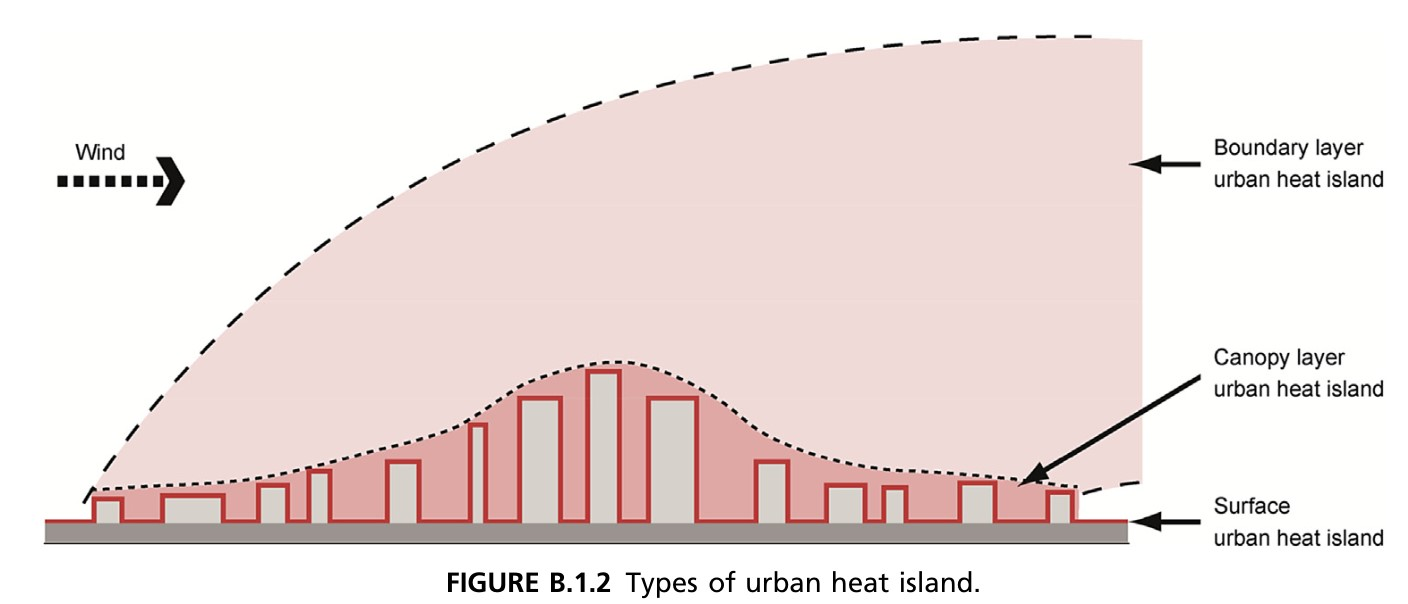
\includegraphics[width=\textwidth]{urban-heat-types}
		\caption{Types of urban heat island. Taken from \textcite{Khan2021}.}
		\label{fig:urban-heat-types}
	\end{figure}
	
	\textbf{Surface urban heat islands} refer to the warmer surface of urbanized areas compared to the temperature of rural surfaces, and is primarily measured by satellite thermal remote sensing data (\cite{Zhou2018}). 
	How hot a surface can reach depends on its properties.
	Dry and exposed surfaces such as roofs and pavements can become significantly hotter than the air, while shaded and moist surfaces remain as hot as the air (\cite{Khan2021}). 
	
	\textbf{Atmospheric urban heat islands} refer to the warmer air temperature of urbanized areas compared to the air temperature of rural areas.
	This category of urban heat island is subdivided into two more classifications:
	the canopy layer urban heat island and the boundary layer urban heat island (\cite{Zhou2018}).
	The canopy layer starts from the ground up to the treetops and rooftops, 
	while the boundary starts from the treetops and rooftops and extends up until point where the urban area does not affect the atmosphere (\cite{Khan2021}).
	There is an intermediate layer known as the roughness sublayer, which starts from ground up to two to five times the height of
	treetops and rooftops.
	In this sublayer, airflow responds to the nature of the individual
	roughness elements themselves (\cite{Oke2017urban}).
	Canopy temperatures are typically measured by sensors from meteorological stations or vehicles,
	while boundary temperatures are measured by sensors from specialized platforms such as tall towers or aircrafts (\cite{Zhou2018}).

\section{Measurement of Urban Heat Islands}
	There are two main ways of conceptualizing the urban heat island.
	The first is the \textbf{urban heat island intensity} (UHII),
	which is determined by the difference between the average and maximum temperature of an urban area, $T_u$, and a rural area, $T_r$ (\cite{Kim2021}):
	\begin{equation}
		\text{UHII} = T_u - T_r.
	\end{equation}
	This gives an indicator of the magnitude of the urban heat island effect in units of $\unit{\degreeCelsius}$.
	Either air temperature or surface temperature may be used.
	The second is using \textbf{energy balance,} which is explained in the next section.
	
	There are three methods in which to study urban heat islands:
	in situ measurements,
	remote sensing observation,
	and modeling (\cite{Bahi2020}).
	In situ instruments come into equilibrium with ambient conditions.
	This response is recorded as the measure of the behavior of the medium.
	Examples include conventional meteorological instruments such as hygrometers, anemometers, and thermometers.
	In situ measurements need the instruments to be situated appropriately in order to extract meaningful information (\cite{Oke2017urban}).
	
	Remote-sensing instruments have sensors that detect radiation from a surface or volume.
	Objects absorb, scatter, and transmit radiation selectively based upon its wavelength.
	Remote sensors tune to different wavelengths and filter different surface types (\cite{Oke2017urban}).
	This retrieves information of a large area at a given time, which is useful for the study of urban heat islands.
	
	Several modeling approaches have been developed to simulate and forecast various atmospheric conditions.
	There are two types of models: atmospheric models and thermodynamic models.
	Atmospheric models simulate regional temperature distribution, while thermodynamic models simulate temperature based on radiative and thermal exchanges between the atmosphere and the urban area.
	Models allow for studies over a larger variety of spatial scales (\cite{Bahi2020}).

\section{Energy Budget and Balance}

	The heating of the Earth is caused by the exchange of energy between the Sun, the Earth's atmosphere, and the Earth's surface.
	The solar rays incident on the Earth, combined with the Earth's rotation, creates a diurnal energy balance (\cite{Wallace2006}).
	The energy is exchanged between layers via radiation, convection and
	conduction.
	These energy exchanges can be associated with an energy flux density, with units $\si{W.m^{-2}}$.
	
	\subsection{Surface Radiation Budget}
		All objects emit radiation, with hotter objects emitting radiation with a shorter wavelength than colder objects.
		The sun emits radiation in the visible spectrum, with the most energy having a wavelength of around $\qty{0.5}{\micro m}$.
		This radiation is referred to as \textit{shortwave radiation} or \textit{solar radiation} (\cite{Oke2017urban}).
		The Earth and its atmosphere also emits radiation but in the infrared range, with the most energy having a wavelength of around $\qty{10}{\micro m}$.
		This radiation is referred to as \textit{longwave radiation} or \textit{terrestrial radiation} (\cite{Oke2017urban}).
		
		\begin{figure}	
			\centering
			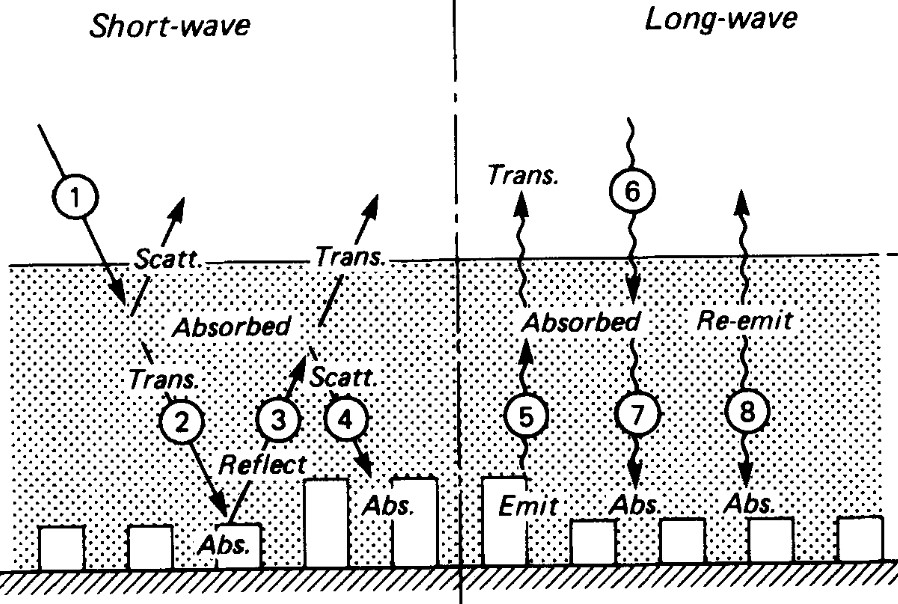
\includegraphics{radiation-budget}
			\caption{Schematic of the radiative processes involved in the radiation budget. See text for explanation of number labels. Taken from \textcite{Oke1982}.}
			\label{fig:radiation-budget}
		\end{figure}
	
		Figure \ref{fig:radiation-budget} depicts a schematic of the fluxes present in the heating of the Earth.
		Shortwave radiation from the sun enters the urban boundary layer.
		Some of the radiation (Fluxes 2 and 4) reach the surface with flux magnitude $Q_{S\downarrow}$.
		The other radiation (Flux 3) is reflected or scattered back upward with flux magnitude $Q_{S\uparrow}$.
		The atmosphere emits longwave radiation, with some (Fluxes 7 and 8)
		reaching the Earth’s surface with flux magnitude $Q_{L\downarrow}$.
		The Earth’s surface also emits longwave radiation (Flux 5) upward with flux magnitude $Q_{L\uparrow}$.
		The net radiation flux $Q^*$ then is given by (\cite{Wallace2006})
		\begin{equation}
			Q^* = Q_{S\downarrow} - Q_{S\uparrow} + Q_{L\downarrow} - Q_{L\uparrow}.
		\end{equation}

	\subsection{Rural Surface Energy Balance}
			
		In a rural environment, the surplus of energy provided by $Q^*$ is shared by the soil and the air.
		Heat is dissipated via conduction to the soil with flux $Q_G$,
			and via convection of sensible and latent heat.
		Sensible heat refers to heat that we can sense.
		Sensible heat flux $Q_H$ refers to the fluid movement of warm air, and is driven by the difference between the surface and the atmosphere.
		Eddies of warm air and cool air are mixed, thus lowering the temperature difference within the atmosphere (\cite{Oke2017urban}).	
		Latent heat refers to the chemical energy of the phase changes of water. 
		There is a latent heat flux $Q_E$ as the water vapor transports the heat to another location.
		Given a mass flux density $E$ of water (with units $\si{kg.m^{-2}.s^{-1}}$), $Q_E$ is calculated by
		\begin{equation}
			Q_E = L_v E,
		\end{equation}
		where $L_v$ is the latent heat of vaporization of water.
		At $\qty{15}{\unit{\degreeCelsius}}$, its value is $\qty{2.464}{MJ.kg^{-1}}$.
		
		By the conservation of energy, each of the mentioned fluxes must balance at the surface.
		Thus,
		\begin{equation}
			Q^* = Q_G + Q_H + Q_E.
		\end{equation}
		This equation is the rural surface energy balance.
		Figure \ref{fig:surface-energy-balance-rural} shows a schematic of the rural surface energy balance equation. The figure treats all heat flux densities as vertical, that is, a one-dimensional view of a horizontal field of grass.
		
		\begin{figure}	
			\centering
			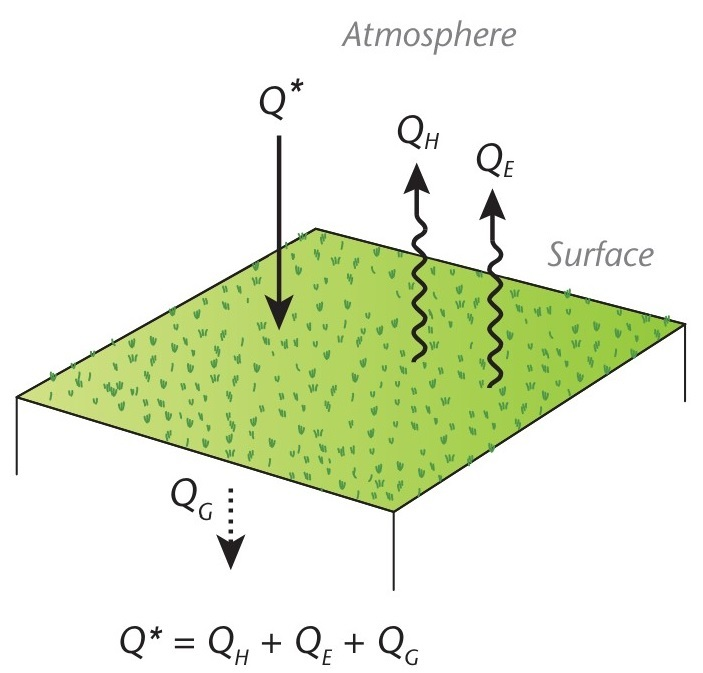
\includegraphics{surface-energy-balance-rural}
			\caption{
				Schematic of the fluxes in the surface energy balance of a rural building-soil-air volume. 
				Arrows are drawn in the direction the corresponding flux is considered positive.
				Taken from \textcite{Oke2017urban}.
			}
			\label{fig:surface-energy-balance-rural}
		\end{figure}
		

	\subsection{Urban Surface Energy Balance}

		An urban environment will modify the energy balance in multiple ways:
		\begin{enumerate}
			\item \textbf{Canyon geometry of buildings.}
			Dense tall buildings create a canyon geometry,
				which causes radiation to get trapped in between the vertical surfaces through multiple reflections.
			This gives a greater absorption of shortwave radiation.
			This also causes a reduction of wind speed, which trap warm air.
			
			\item \textbf{Construction materials.}
			Buildings and paved surfaces are made with materials that have great heat absorption and heat storage.
			
			\item \textbf{Removal of plants and soil.}
			The replacement of plants and moist soil with paved and waterproof surfaces reduces evapotranspiration.
			More of the net radiation flux is thus converted into sensible heat, rather than latent heat.
			
			\item \textbf{Air pollution.}
			A polluted atmosphere has greater absorption and re-emission of radiation, thus increasing longwave radiation flux.
			
			\item \textbf{Anthropogenic heat.}
			There is a release of heat from man-made activities such as from
				the combustion of fuels in vehicles,
				industrial processes, and
				air-conditioning in rooms.
			Humans also release heat and moisture from metabolism, but is not as significant compared to the activities mentioned.
		\end{enumerate}
		A summary of these is shown in Figure \ref{fig:factors-of-urban-heat}.
		
		\begin{figure}
			\centering
			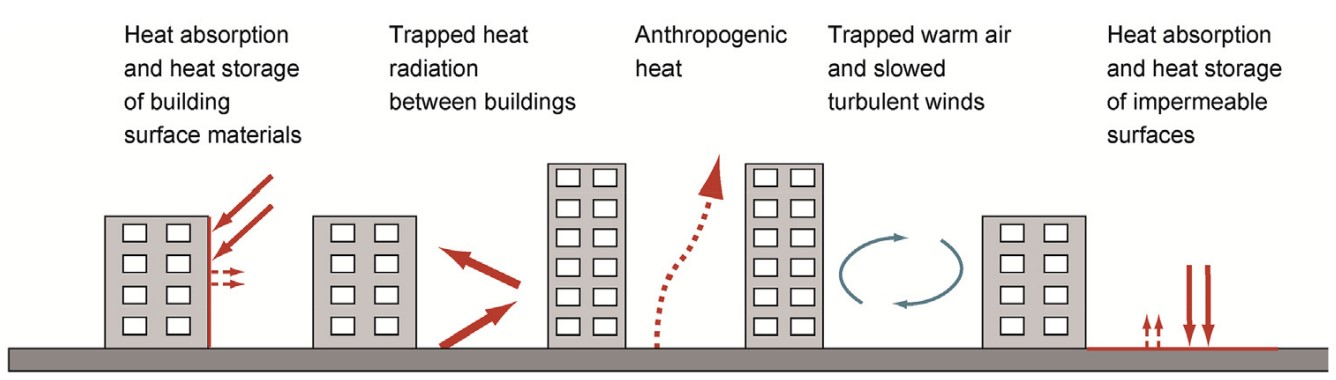
\includegraphics[width=\linewidth]{factors-of-urban-heat}
			\caption{
				Different factors that contribute to heat island formation in the tropical urban area.
				Taken from \textcite{Khan2021}, whom they have modified after \textcite{Kershaw2017}.
			}
			\label{fig:factors-of-urban-heat}
		\end{figure}
		
		Accordingly, modifications in the energy balance equation are needed.
		First, instead of treating the heat flux densities as one-dimensional (along the vertical),
			we consider a three-dimensional volume.
		This way, we can model energy exchanges as occuring on any side of the urban environment, and not just the top.
		We define the bottom of the volume, $z_\text{bot}$, as the depth into the ground wherein there is negligible net conduction over the period of interest.
		We define the top of the volume, $z_\text{top}$, as the top of the roughness sublayer (\cite{Oke2017urban}).
		
		Second, the extra energy sources or energy sinks present in the urban environment need to be accounted for.
		We replace $Q_G$ with $\Delta Q_S$, a term for the storage heat flux.
		We then add a term for anthropogenic heat release flux, $Q_F$, and
			a term for the net advection that lets heat go through the sides of the volume, $\Delta Q_A$.
		
		Applying the modifications mentioned, the energy balance equation thus becomes
		\begin{equation}
			Q^* + Q_F= Q_H + Q_E + \Delta Q_S + \Delta Q_A
		\end{equation}
		for an urban environment (\cite{Oke2017urban}).
		Figure \ref{fig:surface-energy-balance-urban} shows a schematic of the urban surface energy balance equation.
		The $\Delta Q_A$ term may be avoided by assuming or selecting a homogeneous urban surface, wherein horizontal differences are negligible (\cite{Oke2017urban}).
		
		\begin{figure}	
			\centering
			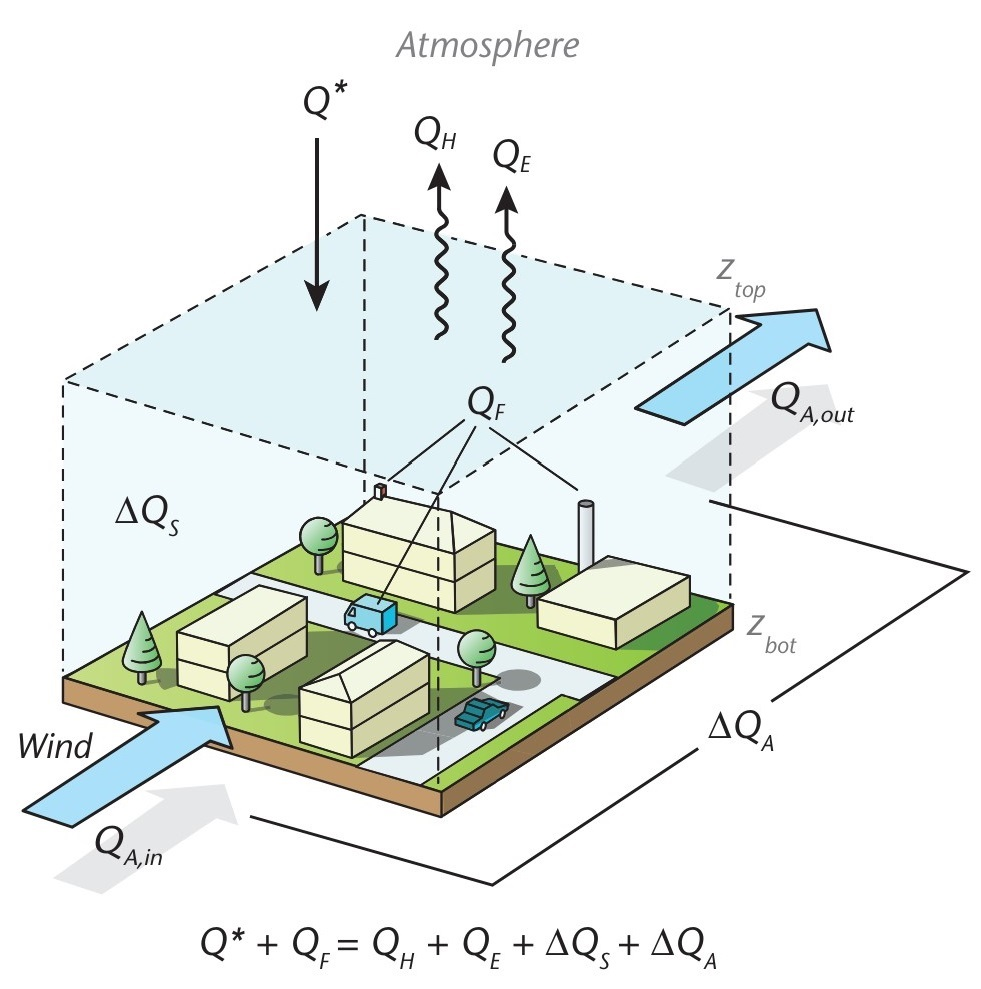
\includegraphics{surface-energy-balance-urban}
			\caption{
				Schematic of the fluxes in the surface energy balance of an urban building-soil-air volume. 
				The volume that extends from the top of the roughness sublayer ($z_\text{top}$) down to a depth where there is no net conduction over the period of interest ($z_\text{bot}$).
				Arrows are drawn in the direction the corresponding flux is considered positive.
				For $\Delta Q_S$ and $\Delta Q_A$, they are positive if the internal energy of the volume increases.
				Taken from \textcite{Oke2017urban}.
			}
			\label{fig:surface-energy-balance-urban}
		\end{figure}
	
\section{Regional Climate Model}
	The study uses the Regional Climate Model (RegCM) in order to study the urban heat island effect.
	RegCM5 is a limited area model for long-term regional climate simulation.
	It is developed by the International Center for Theoretical Physics for long term regional climate
	simulations.
	The latest version, used by this study, is described in detail by \textcite{Giorgi2023}.
	
	\subsection{Inputs and Outputs}
		RegCM needs multiple inputs from global datasets in order to build initial conditions and boundary conditions to run a simulation. RegCM comes with multiple programs to generate inputs from these datasets for the simulation:
		\begin{enumerate}
			\item One is a static surface dataset, which includes the topography and land type classification. 
				The \texttt{domain} program uses this dataset to generate an input and localize the model on a given world region.
			\item Another dataset needed, when using the Community Land Model, is for global land surface characteristics.
				The \texttt{terrain} program uses this dataset to generate inputs for the surface characteristics of the domain, which the Community Land Model needs in order to simulate various land processes.
			\item Another dataset needed is sea surface temperature.
				The \texttt{sst} program uses this to generate inputs for the domain's sea temperature.
			\item One last dataset needed is a global dataset for atmosphere and land temperature, which includes specific humidity, surface air pressure, air temperature, and wind speed.
				The \texttt{icbc} program will use this dataset in order to create the initial conditions and boundary conditions needed by RegCM to run the simulations.
		\end{enumerate}
		The ICTP maintains an online public repository of datasets for use with RegCM (\url{http://clima-dods.ictp.it/regcm4}).
		
		\begin{table}[]
			\caption{
				Surface data required for the Community Land Model and their base spatial resolution.
				Taken from \textcite{Oleson2013}.
			}
			\label{tab:surface-data-clm}
			\centering
			\begin{tabular}{ll}
				\hline \hline
				Surface Field & Resolution                      \\
				\hline
				Percent glacier & 0.05°                         \\
				Percent lake and lake depth & 0.05°             \\
				Percent urban & 0.05°                           \\
				Percent plant functional types (PFTs) & 0.05°   \\
				Monthly leaf and stem area index & 0.5°         \\
				Canopy height (top, bottom) & 0.5°              \\
				Soil color & 0.5°                               \\
				Percent sand, percent clay & 0.083°                           \\
				Soil organic matter density & 0.083°            \\
				Maximum fractional saturated area & 0.125°      \\
				Elevation & 1 km                                 \\
				Slope & 1 km                                     \\
				Biogenic Volatile Organic Compounds & 0.5°      \\
				Crop Irrigation & 0.083°                        \\
				Managed crops & 0.5°                            \\
				Population density & 0.5°                       \\
				Gross domestic production & 0.5°                \\
				Peat area fraction & 0.5°                       \\
				Peak month of agricultural waste burning & 0.5° \\
				\hline
			\end{tabular}
		\end{table}
	
	\subsection{Physics Models}
		RegCM employs a number of physics models which solve a set of dynamical equations describing earth processes.
		These include radiation, convection, turbulent diffusion, moisture, and energy flux exchanges with surface.
		
		These dynamical equations are solved by discretizing. Computed variables are placed on a three-dimensional grid, which can be seen in Figure \ref{fig:regcm-grids}.
		The vertical coordinates of the three-dimensional grid near the ground follow the terrain topology. 
		As the vertical coordinate goes higher, the level slices become flatter.
		The horizontal grids have uniform spacing.
		\begin{figure}	
			\centering
			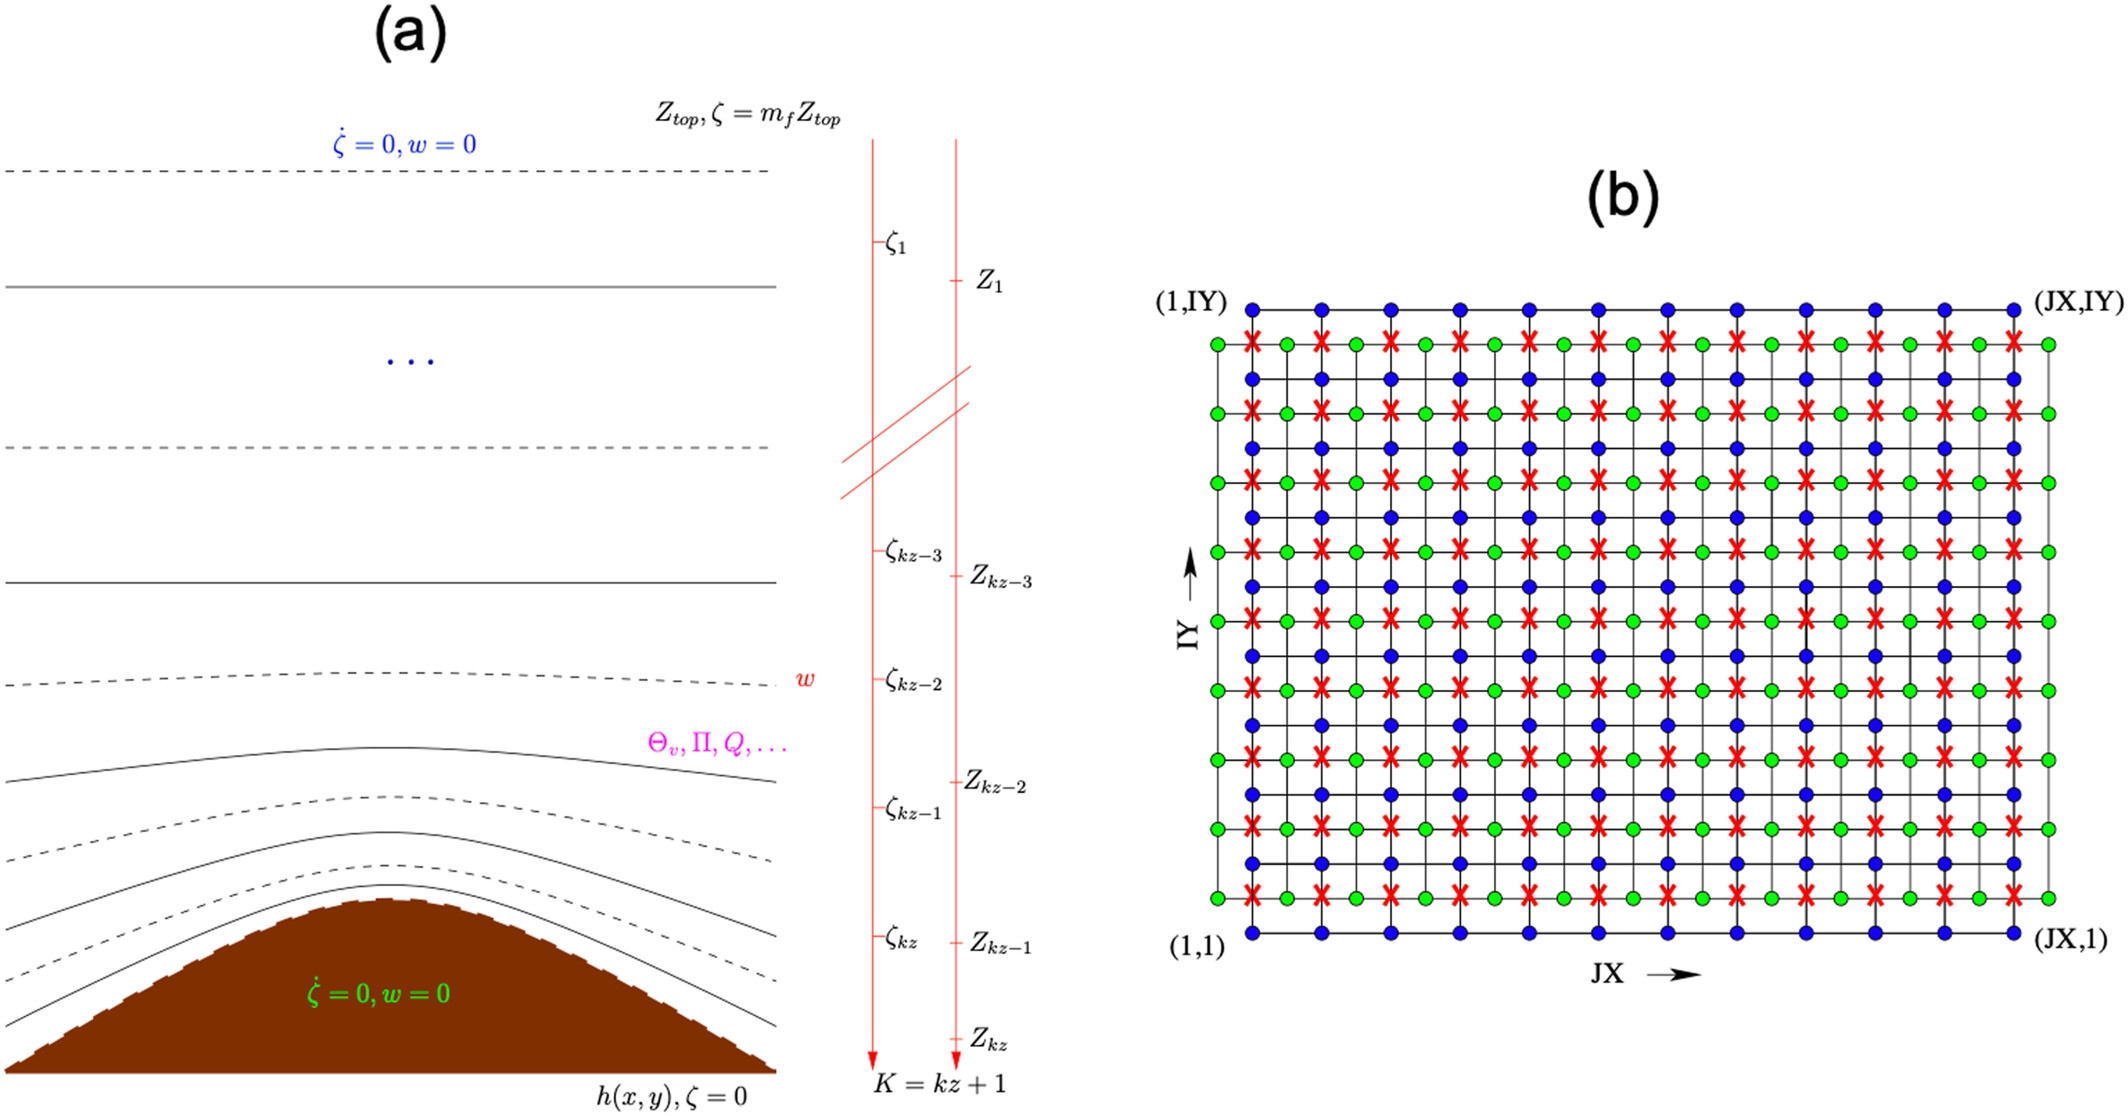
\includegraphics[width = \textwidth]{regcm-grids}
			\caption{
				Vertical and horizontal grid systems used by the MOLOCH dynamical core implemented in RegCM5.
				(a) Terrain following vertical levels and their relationship with atmospheric heights, showing the staggering of the vertical wind (dashed half levels) with respect to the other model status variables (continuous full levels), along with the boundary conditions at the atmosphere top and bottom;
				(b) horizontal staggered Arakawa-C grid.
				Scalar variables are defined at the red X grid points, while the zonal U wind component is defined at the green grid points and the meridional V wind component at the blue grid points.
				Taken from \textcite{Giorgi2023}.
			}
			\label{fig:regcm-grids}
		\end{figure}
		
		
			

	

%\section{Radiative Transfer}
%
%	The sun heats up the atmosphere and surface of Earth through radiative transfer, the transfer of energy via electromagnetic radiation.
%	When radiation interacts with matter, it may either be absorbed, emitted, reflected, scattered, or simply transmitted.
%	The outcome depends on the wavelength of the radiation as well as the properties of the material interacting with the radiation.
%
%	\subsection{Reflection, Scattering, and Albedo}
%	%
%	%As solar radiation travels through the atmosphere,
%	%\blindtext
%	Energy may be returned to space through reflection or scattering.
%	
%	Albedo is defined as the ``ratio of the amount of solar radiation reflected by a surface to the amount received by it'' (\cite{Stewart2012}).
%	
%
%	\subsection{Absorption and Emission}
%	
%	\blindtext
%
%\section{Urban Heat Island}
%
%
%
%	\subsection{Factors Causing Urban Heat Islands}
%	
%	Different climatic and nonclimatic factors are responsible for causing urban heat islands.
%	\citeauthor{Bridgman1995} (\citeyear{Bridgman1995}, as cited in \cite{Khan2021}) lists five major ways in which urbanization can influence a city's climate:
%	\begin{itemize}
%		\item by replacing natural surfaces with asphalts, concrete, and glasses;
%		\item by replacing natural shape with blocky, angular, towering structures;
%		\item by releasing anthropogenic heat into the urban atmosphere;
%		\item by routing flow of surface runoff and preventing infiltration; and
%		\item by emitting pollutants into the urban atmosphere.
%	\end{itemize}